\documentclass[a4paper]{article}

\usepackage[utf8]{inputenc}
\usepackage[portuges]{babel}
\usepackage{a4wide}
\usepackage[margin=1in,includefoot]{geometry}
\usepackage{refstyle}
\usepackage{amsmath}
\usepackage{mathtools}
\usepackage{graphicx}
\graphicspath{ {images/} }

\title{Projeto de Laboratórios de Informática 1\\Grupo 152}
\author{Carlos António Soares de Castro Gomes (A77185) \and Nuno Ricardo Araújo Silva (A78156)}
\date{\today}

\begin{document}

\maketitle

%Cria uma secção chamada resumo em que iremos retratar o trabalho e indicamos a linguagem de programação utilizada e as suas vertentes
\begin{abstract}
Este relatório apresenta o trabalho desenvolvido pelo grupo 152 para
o projeto de Laboratórios de Informática 1 (LI1), do curso Mestrado
Integrado em Engenharia Informática da Universidade do Minho.

O objetivo final consistia em criarmos um jogo clássico, Bomberman. A ideia
geral do jogo é colocar bombas de forma a destruir tijolos e matar os
outros jogadores, e, para isso, tivemos que resolver as Tarefas propostas
pelos responsáveis do projeto.

A linguagem utilizada para atingir este objetivo foi o Haskell com Biblioteca
Gloss.

\end{abstract}

%Irá criar um indice com a descrição de tudo o que se irá abordar
\tableofcontents

%Vai criar uma secção chamada introducao e cria uma label chamada intro para uma possivel referencia futura
\section{Introdução}
\label{sec:intro}


Em linhas gerais, o projeto que nos foi proposto estabelecia criar o jogo clássico, Bomberman, utilizando a
linguagem Haskell e a Biblioteca Gloss, para implementar o jogo.

Este relatório descreve o que foi realizado ao longo do semestre, isto é,
aproximadamente, desde 1 de novembro de 2016 até 02 de janeiro de 2017.

Para atingir o proposto, o trabalho dividiu-se em duas fases, a primeira fase
e segunda fase, cada uma com três tarefas diferentes. Na primeira fase, pretendia-se
criar um mapa, reagir a comandos e codificar o estado. Na segunda
fase baseava-se em reagir à passagem de tempo, implementar o jogo com a Biblioteca
Gloss e implementar um bot que jogue sozinho.

O relatório vai se dividir em três secções, a Descrição do Problema, Concepção da Solução
e Conclusões.

\section{Objetivo - O que foi proposto?}
\label{sec:problema}

Como já foi dito, foi nos proposto criar um jogo clássico, o Bomberman, utilizando
a linguagem Haskell. A ideia geral do jogo é colocar bombas e matar os outros jogadores
até ser o ultimo jogador sobrevivente, mas, para atingir esse propósito, foi dividido
em duas fases, cada uma com três tarefas diferentes com objetivos únicos.

Ao todo, as seis tarefas foram:

\subsection{Primeira Tarefa - Gerar mapas}
\label{subsec:tarefa1}
O objetivo desta tarefa, como o título indica, é gerar mapas recebendo um input, onde
será a dimensão do mapa (número ímpar maior ou igual a cinco) e um número para utilizar
como semente.

\subsection{Segunda Tarefa - Reagir Comandos}
\label{subsec:tarefa2}
O objetivo desta tarefa é, receber um estado de jogo e um comando dum jogador e determinar o que acontece no estado de jogo.

\subsection{Terceira Tarefa - Comprimir o Estado de Jogo}
\label{subsec:tarefa3}
O objetivo desta tarefa é, receber um estado de jogo e tentar implementar um mecanismo de compressão/descompressão, de forma a poupar carácter, e, consequentemente, poupar
espaço em disco quando o estado de jogo for gravado (por exemplo, fazer pausa e continuar o jogo mais tarde).

\subsection{Quarta Tarefa - Reagir à Passagem do Tempo}
\label{subsec:tarefa4}
O objetivo desta tarefa, como o título indica, é reagir ao passar do tempo e determinar o respetivo efeito
no estado de jogo. O jogo será representado no mesmo formato da Tarefa2 (Explicação mais à frente).

\subsection{Quinta Tarefa - Implementação do jogo em Gloss}
\label{subsec:tarefa5}
O objetivo desta tarefa é, implementar o jogo usando a Biblioteca Gloss, onde podiamos
personalizar o jogo ao nosso gosto.

\subsection{Sexta Tarefa - Implementar Estratégia de Combate}
\label{subsec:tarefa6}
O objetivo desta tarefa é, implementar um bot que consiga jogar o Bomberman sozinho, seja qual for
a posição em que o bot estiver.

\section{Concepção da Solução}
\label{sec:solucao}

Para atingirmos o objetivo final, resolvemos as tarefas uma a uma, começando pela Tarefa 1.

\subsection{Primeira Tarefa - Gerar Mapas}
\label{subsec:tarefa1sol}

O objetivo desta tarefa é gerar mapas recebendo um input onde será a dimensão
(número ímpar maior ou igual a cinco) e um número para utilizar como semente e devolve o output que deverá ser um mapa.

Para isso acontecer, em cada célula do mapa pode ser vazia, ou um bloco de pedra indestrutível, ou um
bloco de tijolo destrutível, e em alguns deles, podem esconder powers ups Bombs e
Flames. Então, decidiu-se usar o seguinte formato: o caráter cardinal representa a pedra,'?' representa o tijolo e ' ' o vazio. Depois de representar isso,
é listado os powers ups escondidos em cada linha, e cada power up pode ser representado por: '+' que representa Bombs e '!' que representa os Flames, por esta ordem.

Começamos por apenas desenhar apenas o mapa, sem a lista dos powers ups. Inicialmente, decidimos fazer uma função principal(mapaOriginal) e que chama três funções auxiliares. Porquê? Simplesmenete, observamos que
na primeira/ultima linha só havia cardinais, nas linhas ímpares só havia cardinal na primeira/ultima posição e nas linhas pares havia cardinais só nas posições pares. Mas, depois decidimos
também adicionar uns traços nas posições onde os jogadores começavam, de forma a prevenir que não se adicionava nada e no fim de tudo removia-se os traços, portanto passou a ser usado cinco funções auxiliares.

Depois de termos desenhado o mapa (incluindo os traços, mas ainda sem os '?' e '!'), avançamos para desenhar os powers ups. E, para isso acontecer, definimos a função desenhaPontosMapa que vai começar na posição
0 0 (coluna e linha) e vai percorrer o mapa todo com a lista, e à medida que vai percorrendo e encontra espaços ou power ups, vai apagando os elementos da lista(coordsBombFlares) e, ao mesmo tempo, se encontrar um número entre zero e três, a função adiciona um '?' ao mapa.

Finalmente, depois de estar o mapa desenhado, adicionamos a lista de power ups ao jogo, utilizando a função desenhaBombMap e desenhaFlameMap.

\subsection{Segunda Tarefa - Reagir comandos}
\label{subsec:tarefa2sol}

O objetivo desta tarefa é, receber um estado de jogo e um comando dum jogador e determinar o que acontece no estado de jogo.
Para isso, tivemos que pensar em vários casos, como por exemplo, se o jogador pretende mover para cima e a linha de cima está ocupada, ou se já existe alguma bomba colocada pelo jogador.

Com isso em mente, definimos várias funções (verificaMapaCima, verificaMapaDireita,
verificaMapaEsquerda, VerificaMapaBaixo)
onde recebe as posições iniciais (0,0), a posição do jogador e o mapa
e vai verificar se existe algum bloco de pedra ou tijolo, caso existir a função retorna Falso, caso contrário, tem “caminho livre” para avançar.

Depois de termos feito as funções que verificam se pode mover, fizemos as funções(moveDireita, moveEsquerda,
moveBaixo, moveCima), de modo a alterar a posição do jogador de acordo com o comando que utilizou, mas, primeiro tivemos que verificar se o jogador existia realmente no estado de jogo, pois se não
existisse, o comando não teria efeito no estado de jogo.

Finalmente, definimos a função(apagaPower) que vai apagar a linha do power up do estado de jogo, caso já não exista um '?'/'!' na posição e também definiu-se a função adicionaBomba, caso o jogador
queira colocar uma bomba. A função recebe o número do jogador, o raio (o raio pode variar de acordo com os power ups que o jogador possui), a posição do jogador e o estado de jogo e vai colocar a bomba no estado de jogo, com duração de dez segundos.

\subsection{Terceira Tarefa - Comprimir o Estado de Jogo - Encode }
\label{subsec:tarefa3encode}
O objetivo desta tarefa é, receber um estado de jogo e tentar implementar um mecanismo de compressão/descompressão, de forma a poupar caracter, e, consequentemente, poupar
espaço em disco quando o estado de jogo for gravado (por exemplo, fazer pausa e continuar o jogo mais tarde).

Posto isso, decidimos ir pela maneira mais fácil, guardar a informação toda numa string só. Começamos por meter a dimensão, só bastava contar o número de linhas que começavam com o cardinal e assim tinhamos a nossa dimensão. Depois da dimensão, definimos uma função(posicaoBombsFlames) que vai começar na posição inicial e vai percorrer o mapa todo, e à medida que vai encontrando o '?' adiciona a informação à string. Com isto, só faltava guardarmos informação sobre os Bombs e Flames, então percorremos o mapa e, à medida que ia encontrando a linha que continha informações
sobre os Bombs/Flames, adicionava à string.

Finalmente, só faltava guardar as posições dos jogadores, e fez-se isso através da função posicaoJogador, que percorre o mapa todo e, à medida que encontrava a linha dos jogadores, acrescentava um 'P' para diferenciar da informação da função posicaoBombsFlames e acrescentava a linha do jogador à string.

\subsection{Terceira Tarefa - Comprimir o Estado de Jogo - Decode }
\label{subsec:tarefa3decode}

Tal como foi referenciado na secção \ref{subsec:tarefa3encode}, o objetivo desta tarefa é, receber um estado de jogo e tentar implementar um mecanismo de compressão/descompressão, de forma a poupar caracter, e, consequentemente, poupar
espaço em disco quando o estado de jogo for gravado (por exemplo, fazer pausa e continuar o jogo mais tarde).

Depois de termos feito o encode, tinhamos que arranjar uma alternativa de forma a que (descode(encode mapa)) devolve o próprio mapa original antes de ter feito o encode. A primeira coisa que fizemos, foi aproveitar a dimensão e desenhar apenas o tabuleiro, daí se ter utilizado a função mapaOriginal da Tarefa1. Mas, para utilizarmos essa função, tinhamos que percorrer a string e descobrir a dimensão, felizmente, foi fácil pois era logo o primeiro elemento da string.

Após termos desenhado o tabuleiro, avançamos para desenhar os '?' no tabuleiro, e para isso, tinhamos que guardar as respetivas informações. Sendo assim, utilizou-se a função
arranjarPosicoes em que só deixa a informação dos '?' na string, portanto tinha que se arranjar uma alternativa de guardar a informação na forma duma lista de pares inteiros. Com isso em mente, fez-se a função
converteLista e listaPosicoes. A converteLista vai converter cada posição de '?' em várias linhas diferentes e a listaPosicoes vai converter essa informação para uma lista de pares inteiros. Sucessivamente, fez-se a função desenhaPontosMapa que recebe a lista, com a informação das posições de '?' no tabuleiro, e o tabuleiro.

Por fim, só faltou adicionarmos a lista de power ups, as bombas colocadas e os jogadores existentes ao estado do jogo. Como tal, fez-se getBombsFlames, getBombasColocadas e getPosições. Cada função vai
receber a string e vai identificar quais são as que começam por '+'/'!' ou '*' ou 'P', por esta ordem, e vai adicionar à lista de strings com a função converteLista.

\subsection{Quarta Tarefa - Reagir à Passagem do Tempo}
\label{subsec:tarefa4sol}

O objetivo desta tarefa é, receber um estado de jogo e um comando dum jogador e determinar o que acontece no estado de jogo.
Para isso, tivemos que pensar em vários casos, como por exemplo, se o jogador pretende colocar uma bomba e se lhe é possivel essa mesma função, a explosão duma bomba e os seus efeitos, e o efeito "espiral" que pretende "fechar" o mapa de forma a acabar com o jogo.

Com isso em mente, definimos várias funções (explodeCima, explodeBaixo, explodeHorizontal, apagaPontos, apagaPontosHorizontal, bombasExplodeFinalmente, coordenadaEspiralBaixo, coordenadaEspiralCima, coordenadaEspiralEsquerda, coordenadaEspiralDireita)

onde explodeCima, explodeBaixo, explodeHorizontal, recebe as coordenadas da bomba e verifica o efeito da explosão. Ou seja se destroi algum tijolo, ou power up ou algum jogador.

A função bombasExplodeFinalmente faz com que todas as bombas com o temporizador a 1, explodem.

As funções apagaPontos e apagaPontosHorizontal, verifica atraves dos raios de acção da bomba o que será eleminado. Ou seja se dentro do raio de acção da bomba se encontrar um '\#', não terá qualquer efeito, caso contrário substituirá por ' '.

As funções coordenadaEspiralBaixo, coordenadaEspiralCima, coordenadaEspiralEsquerda, coordenadaEspiralDireita, preenche os espaços com pedras, num efeito tal como o nome indica de "espiral".

Depois de termos feito as funções que verificam se pode mover, fizemos as funções(desenhaEspiral, explodeBomba), de modo a que no mapa comece a surgir o efeito espiral quando o tempo se encontra a ${(n-2)}^2$ segundos de terminar, sendo n o número de linhas. Em que o efeito surge da posição (0,0) e segue na horizontal até encontrar um '\#' de seguida move-se na vertical e assim sucessivamente. Quanto ao explodeBomba irá agrupar os efeitos de cada uma das suas funções auxiliares(explodeCima, explodeBaixo, explodeHorizontal), de forma a surgir uma explosão "completa".

\subsection{Quinta Tarefa - Implementação do jogo em Gloss}
\label{subsec:tarefa5sol}

Nesta tarefa pretende-se implementar a Biblioteca Gloss de forma a construir uma interface e existir uma via de interação entre o utilizador e o programa.

Dessa forma definimos algumas funções entre as quais insereJogador, reageTempo, reageComando, desenhaEstado, desenhaMapa, desenhaTijolo, desenhaBomba, variosJogadores.

Algumas funções como insereJogador ou reageTempo ou reageComando, irão respetivamente, inserir no sistema os jogadores, a alteração do estado do jogo a cada n segundos e alterar o estado de jogo sempre que é ordenado uma certa acção, por exemplo colocar uma bomba.

A função desenhaEstado, variosJogadores, desenha as interações do jogo como as bombas nas posições pretendidas.

A função desenhaMapa, desenha o mapa em si através das funções auxiliares desenhaLinha(desenha uma linha inteira de imagens), desenhaLinha1(desenha a imagem na primeira e na ultima posição), desenhaLinha2(desenha as imagens nas posições pares).

A função desenhaBomba, desenha todas as bombas colocadas no estado de jogo, utilizando uma função auxiliar denominada desenhaBombaImagem que desenha todas as bombas numa linha.

A função desenhaTijolo, desenha um tijolo nas posições onde se encontra um '?', esta função é auxiliada pela função desenhaTijoloImagem, que desenha todos os tijolos numa linha.

A função variosJogadores irá adicionar todos os jogadores existentes no estado de jogo.

\begin{center}
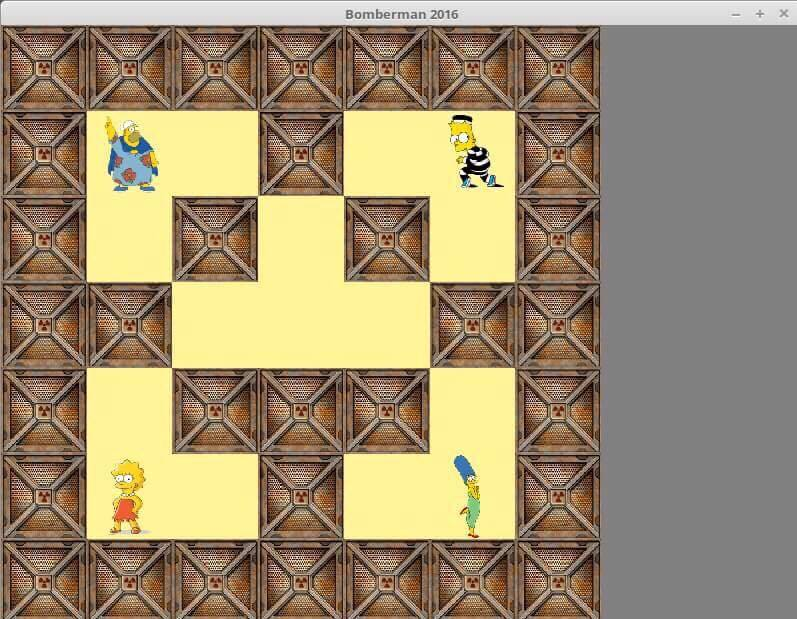
\includegraphics[width=15cm, height=10cm]{tabuleiro}
Imagem referente ao nosso tabuleiro.
\end{center}

\subsection{Sexta Tarefa - Implementar Estratégia de Combate}
\label{subsec:tarefa6sol}

O objetivo desta tarefa é, implementar um bot que consiga jogar o Bomberman sozinho, seja qual for
a posição em que o bot estiver.

Sendo assim criamos funções tais como verificaBombaColocada, verificaBombaColocadaU, verificaBombaColocadaD, verificaBombaColocadaL, verificaBombaColocadaR, que irão verificar se o bot esta em cima duma bomba, ou se existe alguma bomba prestes a rebentar acima, abaixo, à esquerda ou à direita do bot. Foi criada tambem uma função que verifica a existência de algum jogador nas proximidades do bot, chamada verificaBombaMata.

Criamos tambem uma função denominada verificaComandos que verifica os comandos possíveis em cada posição que o jogador estiver. Por exemplo, se o jogador 0 estiver na posição inicial, só vai ser possivel mover-se para a direita/baixo ou colocar bomba. Para tal são utilizadas funções auxiliares chamadas verificaBombaColocada, listaBombas, converteLista, getBombasColocadas, verificaBombaColocadaU, verificaBombaColocadaD, verificaBombaColocadaL, verificaBombaColocadaR, verificaBombaMata, listaCoordsJog.

Por fim utilizamos uma função retirada do Google, denominada pick, que tem por objetivo escolher um elemento aleatório da lista. Ou seja o bot tomará aleatoriamente as decisões possiveis para cada situação.

\subsection{Testes}

Tal como foi referenciado na secção \ref{subsec:tarefa3encode}, guardamos a informação toda do mapa numa só string.

Para tal utilizaremos, por exemplo, o mapa de dimensão 9 e com seed 0, a representação do mapa será:
\begin{verbatim}
["#########",
"# #",
"# #?#?# #",
"# ? ? #",
"#?# # #?#",
"# ? ? #",
"# #?#?# #",
"# ?? #",
"#########",
"+ 5 2",
"+ 3 3",
"! 5 5"]
\end{verbatim}

Depois de ter sido processado pelo o encode, a informação do mapa estará numa string compacta e reduzida, "9/3 2/5 2/3 3/6 3/1 4/7 4/2 5/5 5/3 6/5 6/3 7/4 7/+ 5 2/+ 3 3/! 5 5/".

Com isto verificamos a presença de indicadores chave do mapa como a dimensão, tijolos(representados pelas suas coordenadas e espaçados por '/') e power ups(representados pelas suas coordenadas e o seu caráter característico).

\section{Conclusões}
\label{sec:conclusao}

Neste trabalho que foi feito, concluimos que a experiência foi positiva, apesar dos resultados não terem sidos como esperados em certos aspectos entre os quais, na Tarefa 3 e na Tarefa 5. Em que a compressão/descompressão esperada não foi similar ou ate mesmo próxima aos resultados obtidos. Quanto à Tarefa 5, apesar de não apresentar qualquer erro de syntax obtivemos uma má representação do mapa pois os tijolos e as pedras têm as mesma imagem ao representa-las.
Quanto à linguagem de programação utilizada na concepção na nossa opinião sincera, achamos que não seria a mais fácil para este fim mas que atraves dela ganhamos raciocinio e aprendemos uma nova forma de pensar nos problemas que nos poderão vir a ser uteis futuramente.

\end{document}